\documentclass[12pt]{article}
\usepackage[utf8]{inputenc}
\usepackage[T2A]{fontenc}
\usepackage[russian]{babel}
\usepackage{amsmath}
\usepackage{amssymb}
\usepackage{dsfont}
\usepackage[dvipsnames]{xcolor}
\usepackage{setspace}
\usepackage{multirow}
\usepackage[a4paper, outer=1.5cm, inner=1.5cm, top=1cm, bottom=1cm]{geometry}
\usepackage{graphicx}
\usepackage{skull}
\usepackage{wasysym}
\usepackage{float}
\graphicspath{{.images/}}
\usepackage{hyperref}
\hypersetup{colorlinks=true, linkcolor=blue, filecolor=magenta, urlcolor=cyan}
\usepackage[firstpage]{draftwatermark}
\SetWatermarkText{
    $\qquad\qquad\qquad\qquad\qquad$\parbox{7cm}{\begin{center}
    
\includegraphics[width = 0.08\textwidth]{lion-logo.png}\bigskip\\~\bigskip\\~\vspace{-24mm}\\~\end{center}}
}
\SetWatermarkAngle{0}
\SetWatermarkScale{1.5}
\usepackage{etoolbox}

\newtoggle{ifsolved}
\newtoggle{needhelp}
\newcounter{num}
\setcounter{num}{1}

\newcommand{\newnum}{\par\textbf{\textnumero\arabic{num}}\stepcounter{num}}
\newcommand{\sol}{\vspace{3mm}\par\textbf{Решение: }}
\newcommand{\ans}{\vspace{3mm}\par\textbf{Ответ: }}
\newcommand{\hint}{\vspace{3mm}\par\textbf{Подсказка: }}
\newcommand{\mode}[1]{
\ifstrequal{#1}{0}{\togglefalse{ifsolved}\togglefalse{needhelp}}{\ifstrequal{#1}{1}{\togglefalse{ifsolved}\toggletrue{needhelp}}{\ifstrequal{#1}{2}{\toggletrue{ifsolved}\togglefalse{needhelp}}{\toggletrue{ifsolved}\toggletrue{needhelp}}}}} %if 0 - if 1 - if 2 - else
%\newenvironment{problem}[8]{%#1, #2, #3
%\parbox{\linewidth}{\vspace{4mm}\ifstrequal{#4}{(лёгкая)}{\newnum\textbf{.}}{\newnum\textbf{*.} } \\ #5}
%\iftoggle{ifsolved}{\sol #6}{}
%\iftoggle{ifsolved}{\ans #7}{}
%\iftoggle{needhelp}{\hint #8}{}}

\newenvironment{problem}[8]{%#1, #2, #3
\parbox{\linewidth}{\vspace{5mm}\ifstrequal{#4}{(лёгкая)}{\newnum\textbf{.}}{\newnum\textbf{*.} } \\ #5}
\iftoggle{ifsolved}{\sol #6}{}

\iftoggle{ifsolved}{\parbox{\linewidth}{\ans #7}}{}
\iftoggle{needhelp}{\parbox{\linewidth}{\hint #8}}{}}

\newenvironment{mylist} %custom list
{ \begin{itemize}
    \setlength{\itemsep}{0pt}
    \setlength{\parskip}{0pt}
    \setlength{\parsep}{0pt}     }
{ \end{itemize}                  }

\newenvironment{homeass}[1]{\vspace*{-1.5cm}
\iftoggle{ifsolved}{
    \section*{\center{Решение домашнего задания к #1.}}
}{
    \section*{\center{\textcolor{Sepia}{Домашнее задание к #1}}}
} \vspace{7mm}\large}

\parindent=0pt
\pagestyle{empty}
%$\!$[\arabic{class}.\arabic{num}]
%\ifnumcomp{\value{counter}}{>}{1}{true}{false}
%\definecolor{Gray}{gray}{0.9}
%\definecolor{mypink}{RGB}{219, 48, 122}
%\newcolumntype{g}{>{\columncolor{Gray}}p{2.8cm}}

\begin{document}
\large
\mode{7}
%0 for problems without hints
%1 for problems + hints
%2 for problems + solutions + answers
%else: show all

{\centering\section*{СПИСОК ЗАДАЧ}}

{\centering\subsection*{\smallskip\\\textcolor{green}{\textbf{Полезные вещи, которые можно и нужно копипастить:}}}}

\subsection*{\textcolor{Emerald}{\textbf{Полезные шпаргалки по LaTeXу:}}}

\textbf{Пример вставки рисунка:}

\begin{minipage}{\linewidth}
    \begin{minipage}{0.54\linewidth}
    см. рисунок справа\\
    Текст к собственно пикче, примерно всегда это либо развёрнутое описание, либо большая часть решения задачи --- стремимся экономить пространство, если это можно сделать.
    \end{minipage}
    \hspace{0.05\linewidth}
    \begin{minipage}{0.4\linewidth}
    \begin{figure}[H] 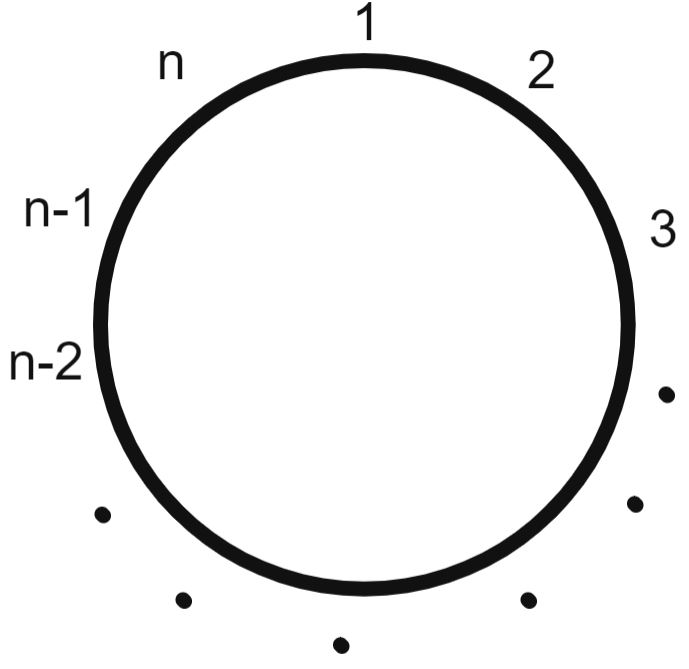
\includegraphics[width=\linewidth]{sol3} %тут поменять имя пикчи
    \end{figure}
    \end{minipage}
\end{minipage}

\textbf{Дефолтные математические знаки и символы:}\\
$\geqslant$,
$\leqslant$,
$a^{b}$,
$x_{i}$,
$\sqrt{a}$,
$\frac{a}{b}$,
$\displaystyle \frac{a}{b}$,
$\cdot$
$\;\Rightarrow\;$,
$\;\Leftrightarrow\;$,
$1{,}2$.
О промежутках:
$a\!b$,
$a\,b$,
$a\:b$,
$a\;b$,
$a\quad b$.

\textbf{Стандартные система и совокупность уравнений / неравенств:}\\
$\left\{
\begin{aligned}
f(x) &= 0 \\
g(x) &= 1
\end{aligned}\right.$

$\left[\begin{aligned}
&\left\{\begin{aligned}
f(x) &\geqslant a \\
g(x) &= b
\end{aligned}\right.\\
&\left\{\begin{aligned}
f(x) &< a \\
g(x) &= -b
\end{aligned}\right.
\end{aligned}\right.$

\subsection*{\textcolor{Emerald}{\textbf{Не математическое, но полезное:}}}
% комментарий в любом месте документа, который нигде не будет видно. Можно использовать для написания заметок-вопросов по задачам
\textbf{Пример таблицы:}

\begin{tabular}{|c|c|c|}
\hline
    $a$ & $b$ & текст
\\\hline
    $c$ & $d$ & мораль
\\\hline
\end{tabular}\\

\textbf{Отступы:} между\smallskip\\ строками\medskip\\ \textbf{Тире} --- это три дефиса.\\
\textbf{Списки:}
\begin{mylist}
\item [$\bullet$] это был пункт а
\item [2)] а это уже пункт номер 2 с изменённым заголовком
\end{mylist}

\subsection*{\textcolor{Emerald}{\textbf{Всё, неупомянутое выше (или если просто что-то не так):}}}
\begin{mylist}
\item [$\bullet$] Решение отдельных вопросов касательно ТеХа нужно искать в \href{https://www.mccme.ru/free-books/llang/newllang.pdf}{Львовском}.

\item [$\bullet$] Найти произвольный символ, который нужен, можно в \href{http://detexify.kirelabs.org/classify.html}{Detexify}.

\item [$\bullet$] Если возникли сомнения при решении, ответ практически ко всем задачам можно проверить с помощью \href{https://www.wolframalpha.com/}{WolframAlpha}.

\item [$\bullet$] Если в задаче нужно создать картинку, то лучше пока отложить эту задачу. Все графики планируется централизованно нарисовать (или перерисовать) в геогебре.

\item [\textcolor{brown}{\textbf{!!}}] Важно ставить \textcolor{red}{\textbf{$\spadesuit$}}
(или просто red) в тело задачи в случае серьёзных вопросов к решению и какой-то вопиющей лажи.

\item [\textcolor{brown}{\textbf{!!}}] Важно ставить \textcolor{olive}{\textbf{$\spadesuit$}}
(или просто olive) в тело задачи в случае не самого удачного текста и кривых отступов.
\end{mylist}

\subsection*{\textcolor{Violet}{\textbf{Комментарии:}}}% а также невидимые комментарии - так можно оставлять заметки-вопросы прямо в задаче, чтобы потом было понятно, в чём вопрос.
\begin{mylist}
\item [$\skull$] Переставлять задачи местами --- очень плохая идея.

\item [$\smiley$] При двойном клике по тексту pdf справа происходит автоматический переход к этому месту в латех-коде, а для обратного перехода можно нажать стрелку вправо (висит сверху между pdf и латех-кодом).

\item [$\smiley$] Если есть размышления, дописывать red/olive к задаче или не дописывать, то лучше всё-таки дописать.

\item [$\skull$] Самое плохое, что можно сделать --- написать в любое поле из трёх (НаписанноеРешение/ВерныйОтвет/Подсказка) только половину того, что надо, никак это не отметить, и потом пойти дальше.\\ Нужно в этот момент писать red/olive в случайном месте задачи, чтобы потом вычислить это с помощью Ctrl+F по всему документу (и это то, что потом будет делаться долго и тщательно)
\end{mylist}

\newpage
\setcounter{num}{1458}

\hypertarget{10.1}{{\centering\section*{\bigskip\\\textcolor{Blue}{\hyperlink{start2}{\textcolor{Blue}{10.1}} Тригонометрические функции.}\vspace{-5mm}}}}

\begin{problem}{Синус и косинус, их свойства.}{10.1.4}{9D}{(лёгкая)}
{Известно, что для некоторого угла $\gamma$ косинус и синус имеют разные знаки.\\
В какой четверти может находиться этот угол?}
{Возможны два варианта: или косинус положителен, а синус отрицателен, или наоборот, отрицателен косинус, а синус положителен. В первом случае координата по $x$ положительна, а по $y$ отрицательна $\Rightarrow$ это IV четверть.\\ Во втором случае $x$-координата отрицательна, а $y$-координата положительна $\Rightarrow$ это II четверть.}
{Это либо II, либо IV четверть.}{$\cos$ по горизонтали, $\sin$ по вертикали.}
\end{problem}

\begin{problem}{Синус и косинус, их свойства.}{10.1.4}{9D}{(лёгкая)}
{Известно, что косинус угла равен 1/2.\\
В какой четверти может находиться этот угол и чему может быть равен его синус?

}
{Косинус угла положителен, а значит $x$-координата получающейся точки положительна, поэтому она и угол находятся в I или IV четверти (см. рисунок)\vspace{-4mm}\\\begin{minipage}{\linewidth}
    \begin{minipage}{0.65\linewidth}
    ~\vspace{1mm}\\
    Для этого угла $\alpha$, где бы он ни находился, выполнено основное тригонометрическое тождество:\\ $\cos^2 \alpha + \sin^2 \alpha = 1$ (оно же теорема Пифагора).\medskip\\
    Отсюда $\sin^2 \alpha = 1 - \left(\frac12\right)^2 = 1 - \frac14 = \frac34 \;\Rightarrow\; \sin\alpha = \pm\frac{\sqrt{3}}{2}$.\medskip\\ Как мы можем видеть, оба варианта возможны: в I четверти синус положителен, а в IV~--- отрицателен.
    \end{minipage}
    \hspace{0.05\linewidth}
    \begin{minipage}{0.3\linewidth}\begin{figure}[H] 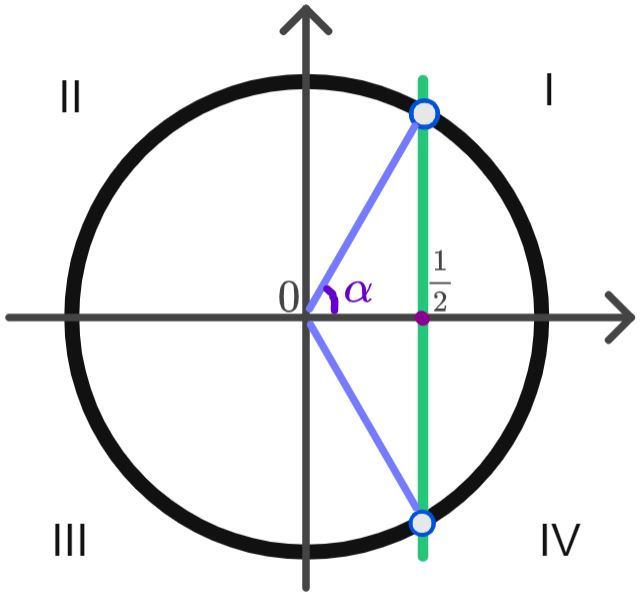
\includegraphics[width=\linewidth]{sol37}\end{figure}\end{minipage}
\end{minipage}\vspace{-2mm}}
{Угол находится в первой или четвёртой четверти, его синус равен $\pm\frac{\sqrt{3}}{2}$.}{Основное тригонометрическое тождество выполнено для всех углов.}
\end{problem}

\begin{problem}{Синус и косинус, их свойства.}{10.1.4}{9D}{(лёгкая)}
{Для некоторого угла, находящегося во второй четверти, известен косинус:\\ он равен $ -\frac{12}{13}$. Найти, чему равен синус этого угла.}
{Так как этот угол $\alpha$ находится во второй четверти, его синус должен быть положителен. Используем теорему Пифагора: $\, \displaystyle \sin^2 \alpha + \cos^2 \alpha = 1 \;\Rightarrow\;$ \\ $ \Rightarrow\; \vphantom{\Bigr(}\sin^2 \alpha = 1 - \left(-\frac{12}{13}\right)^2 = 1 - \frac{144}{169} = \frac{169 - 144}{169} = \frac{25}{169}$. Следовательно, $\sin \alpha = \frac{5}{13}$. (в данном случае $-\frac{5}{13}$ является посторонним корнем, так как нам известно, что синус положителен).}
{Синус этого угла равен $\frac{5}{13}$.}{Положительны или отрицательны синусы углов II четверти?}
\end{problem}

\begin{problem}{Синус и косинус, их свойства.}{10.1.4}{9D}{(лёгкая)}
{Найти $\cos \alpha$, если $\sin \alpha = \frac{8}{17}\,$ и $\,\frac{\pi}{2} < \alpha < \pi$.}
{НаписанноеРешение}
{ВерныйОтвет}{Подсказка}
\end{problem}

\begin{problem}{Синус и косинус, их свойства.}{10.1.4}{9D}{(лёгкая)}
{Известно, что $\displaystyle \cos\beta = -\frac{35}{37}$, и угол $\beta$ находится то ли в III, то ли в IV четверти. Чему равен $\sin\beta$?}
{Согласно теореме Пифагора, $\cos^2 \beta + \sin^2 \beta = 1$, откуда имеем \\ $\sin^2 \beta = 1 - \cos^2 \beta = 1 - \left(-\frac{35}{37}\right)^2 = 1 - \frac{35^2}{37^2} = \frac{37^2 - 35^2}{37^2} = \frac{(37 - 35)(37 + 35)}{37^2} = \frac{144}{37^2} = \frac{12^2}{37^2}$. Значит, $\sin \beta = \pm \frac{12}{37}$. Нам известно, что угол $\beta$ находится в третьей или четвёртой четверти. Однако обе эти четверти находятся ниже оси абсцисс, а значит синус угла $\beta$ обязан быть отрицательным! Таким образом, $\sin \beta = -\frac{12}{37}$.}
{$\sin \beta = -\frac{12}{37}$.}{Каков знак синуса?}
\end{problem}

\begin{problem}{Синус и косинус, их свойства.}{10.1.4}{9D}{(лёгкая)}
{Известно, что $\displaystyle \sin\gamma = \frac{20}{29}$, а в какой четверти находится угол, неизвестно.\\ Чему может быть равен $\cos\gamma$?}
{Независимо от того, в какой четверти находится угол, для образуемого им прямоугольного треугольника должна быть выполнена теорема Пифагора:\smallskip\\ $\cos^2 \gamma + \sin^2 \gamma = 1 \;\Rightarrow\; \cos^2 \gamma  = 1 - \left(\frac{20}{29}\right)^2 = \frac{29^2 - 20^2}{29^2} = \frac{(29 - 20)(29 + 20)}{29^2} = \frac{9 \cdot 49}{29^2} = \frac{3^2 \cdot 7^2}{29^2} \;\Rightarrow\; \cos\gamma = \pm\frac{21}{29}$. Поскольку четверть, как следует из условия, может быть любой, косинус может быть как отрицательным, так и положительным.}
{$\cos\gamma = \pm\frac{21}{29}$.}{Используй основное тригонометрическое тождество.}
\end{problem}

\begin{problem}{Синус и косинус, их свойства.}{10.1.4}{9D}{(лёгкая)}
{Известно, что $\displaystyle \cos\varphi = -0{,}96$, а угол находится в III четверти.\\ Чему равен $\sin\varphi$?}
{Согласно теореме Пифагора (основному тригонометрическому тождеству), $\sin^2\varphi + \cos^2\varphi = 1$, откуда $\sin^2\varphi = 1 - \cos^2\varphi = 1 - (-0{,}96)^2 = 1 - (-\frac{24}{25})^2 = $ \\ $1 - \frac{576}{625} = \frac{625 - 576}{625} = \frac{49}{625}$. Нам известно, что угол находится в III четверти, а значит, и косинус, и синус отрицательны. Следовательно, $\sin^2\varphi = \frac{49}{625} \;\Rightarrow\; \sin\varphi = -\sqrt{\frac{49}{625}} = -\frac{7}{25} = -0{,}28$. Таким образом, $\sin\varphi = -0{,}28$.}
{$\sin\varphi = -0{,}28$.}{Используй основное тригонометрическое тождество.}
\end{problem}

\begin{problem}{Синус и косинус, их свойства.}{10.1.4}{9D}{(лёгкая)}
{В треугольнике $ABC$ угол $C$ равен $90^{\circ}$, $CH$~--- высота, $BC = 4$, $CH = \sqrt{15}$.\\ Найти $\sin A$.}
{\vspace{-4mm}\\\begin{minipage}{\linewidth}
    \begin{minipage}{0.66\linewidth}
    ~\vspace{1mm}\\
    В любой геометрической задаче первым делом нужно построить правильный чертёж: он изображён на рисунке справа.\smallskip\\ Интересующий нас угол отмечен фиолетовым~--- это угол $CAB$ (угол $A$).\\ Угол $BCH$ также равен углу $A$ (так как он также дополняет до $90^{\circ}$ угол $ACH$). Следовательно, можно вместо синуса угла $A$ найти $\sin \angle BCH$.\\ По определению, синус угла в прямоугольном треугольнике равен отношению противолежащего катета к гипотенузе, то есть, в нашем случае, $\frac{BH}{BC}$.\smallskip\\
    Согласно теореме Пифагора, $BH = \sqrt{BC^2 - CH^2} = \sqrt{16 - 15} = 1$.\\ Поэтому $\sin A = \sin \angle BCH = \frac{BH}{BC} = \frac{1}{4} = 0{,}25$.
    \end{minipage}
    \hspace{0.05\linewidth}
    \begin{minipage}{0.27\linewidth}\begin{figure}[H] 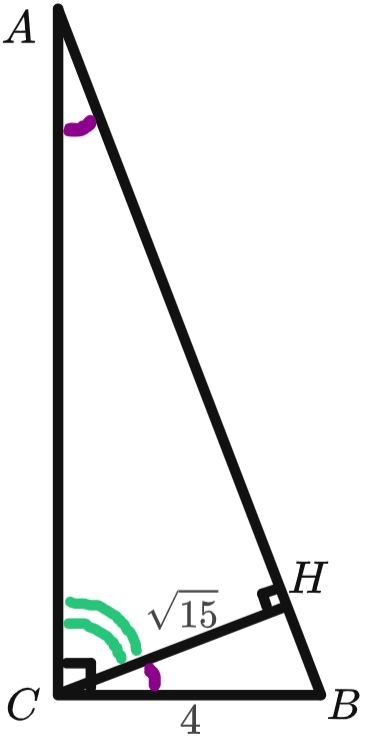
\includegraphics[width=\linewidth]{sol39}\end{figure}\end{minipage}
\end{minipage}\vspace{-2mm}}
{$\sin A = 0{,}25$.}{Какой ещё угол на рисунке равен углу $A$? Обоснуй и реши задачу.}
\end{problem}

\begin{problem}{Синус и косинус, их свойства.}{10.1.4}{9D}{(лёгкая)}
{В треугольнике $DEF$ угол $F$ равен $90^{\circ}$, $\cos D = 0{,}4$, $EF = 3\sqrt{21}$. Найти $DE$.}
{\vspace{-4mm}\\\begin{minipage}{\linewidth}
    ~\vspace{2mm}\\
    \begin{minipage}{0.76\linewidth}
    В первую очередь рисуем треугольник (см. рисунок справа).\\ Пусть длина $DE$ равна $x$. Тогда, по определению косинуса угла в прямоугольном треугольнике, $\cos D = \frac{DF}{DE}$, откуда $DF = \cos D \cdot DE = 0{,}4x$. Таким образом, все стороны этого треугольника выражены через $x$.\\ Но поскольку треугольник $DEF$~--- прямоугольный, для него выполнена теорема Пифагора: $DE^2 = DF^2 + EF^2 \;\Rightarrow\; $ $x^2 = 0{,}16x^2 + 9 \cdot 21 \;\Rightarrow\; 0{,}84x^2 = 9 \cdot 21 \;\Rightarrow\;$ $x^2 = 9 \cdot 21 \cdot \frac{100}{84} = 9 \cdot 25$. Следовательно, $x = 3 \cdot 5 = 15$. Сторона $DE$ равна 15.
    \end{minipage}
    \begin{minipage}{0.23\linewidth}\begin{figure}[H] 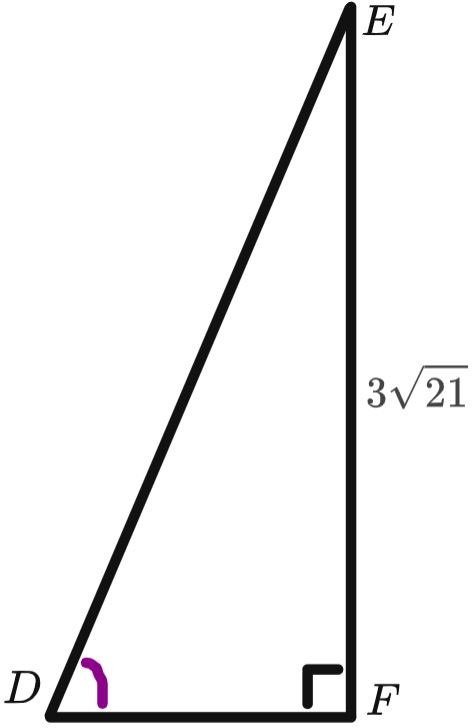
\includegraphics[width=\linewidth]{sol46}\end{figure}\end{minipage}\vspace{-3mm}
\end{minipage}}
{Сторона $DE$ равна 15.}{Изобрази треугольник и обозначь искомую сторону за $x$.}
\end{problem}

\begin{problem}{Тангенс и котангенс, их свойства.}{10.1.5}{9D}{(лёгкая)}
{В поле пересекаются две дороги~--- прямая, которая задаётся уравнением $y = \sqrt{3}x - 2$ и прямая $y = 0$. Под каким углом они пересекаются?}
{НаписанноеРешение}
{ВерныйОтвет}{Подсказка}
\end{problem}

\begin{problem}{Тангенс и котангенс, их свойства.}{10.1.5}{9D}{(лёгкая)}
{Найти значение выражения $\tg\left(-\frac{13\pi}{6}\right) \cdot \sin\left(-\frac{13\pi}{3}\right)$.}
{НаписанноеРешение}
{ВерныйОтвет}{Подсказка}
\end{problem}

\begin{problem}{Тангенс и котангенс, их свойства.}{10.1.5}{9D}{(лёгкая)}
{Вычислить значение выражения $\tg\frac{\pi}{6} \cdot \cos\frac{\pi}{4} \cdot \sin\frac{\pi}{3}$.}
{Все значения углов в задаче, $\frac{\pi}{6}$, $\frac{\pi}{4}$, $\frac{\pi}{3}$~--- табличные.\\ Получаем: $\displaystyle \tg\frac{\pi}{6} \cdot \cos\frac{\pi}{4} \cdot \sin\frac{\pi}{3} = \frac{\sin\frac{\pi}{6}}{\cos\frac{\pi}{6}} \cdot \cos\frac{\pi}{4} \cdot \sin\frac{\pi}{3} = \frac{\frac12}{\frac{\sqrt{3}}{2}} \cdot \frac{\sqrt{2}}{2} \cdot \frac{\sqrt{3}}{2} = \frac{\sqrt{2}}{4}$.\vspace{-3mm}\\}
{$\displaystyle \tg\frac{\pi}{6} \cdot \cos\frac{\pi}{4} \cdot \sin\frac{\pi}{3} = \frac{\sqrt{2}}{4}$.}{Все углы в задаче табличные.}
\end{problem}

\end{document}